\documentclass[english]{article}

\usepackage{babel}
\usepackage{graphicx}
\usepackage{times}
\usepackage{pifont}
\usepackage[margin=1in]{geometry}
\usepackage{eurosym}
\usepackage{fancyhdr}
\usepackage[hidelinks]{hyperref}
\usepackage{gensymb}
\usepackage{float}
\pagestyle{fancy}
\usepackage{mathtools}
\fancyhf{}


%HEADER
%**************************************************************************************
\pagestyle{fancy}
\fancyhf{}
%**************************************************************************************
\lhead{Cable radar (TDR)}		 	 
\rhead{Laboratory Work in Telecommunications} 
\lfoot{EFA12SF}
\cfoot{\thepage}
\rfoot{Dmitry Boronin\\ Nikolay Arsenov\\ Alexey Tukalo}
%**************************************************************************************

\date{}
\setlength\parindent{0pt}

\begin{document}

\title{\vspace{2in}Cable radar (TDR)\\
\small for Laboratory Work in Telecommunications\\
\vspace{0.5in}
\includegraphics{savonia.jpg}}

\nopagebreak
\maketitle


\vspace{3in}

\author{
\begin{flushright}
Dmitry Boronin, Nikolay Arsenov, Alexey Tukalo,\\
EFA12SF,\\
Information Technology,\\
Savonia University of Applied Sciences
\end{flushright}
}

\date{\today}
\thispagestyle{empty}

\newpage
\setcounter{page}{1}
\setcounter{tocdepth}{2}
\tableofcontents

\newpage

%MAIN CONTENT ******************************************************************************************************************

\section{Introduction}
A Cable radar or a time-domain reflectometer (TDR) is an instrument that is used to look for location of different faults in metallic cables. There is more accurate versions of the device which can be applied to determine location of problems in printed circuit boards.\\\\
The device transmits a signal via wire and listens for reflections which are produced by interaction of uneven impedance.
\subsection{Usage}
Time domain reflectometers are commonly used for in-place testing of very long cable runs, where it is impractical to dig up or remove what may be a kilometers-long cable. They are indispensable for preventive maintenance of telecommunication lines, as TDRs can detect resistance on joints and connectors as they corrode, and increasing insulation leakage as it degrades and absorbs moisture, long before either leads to catastrophic failures. Using a TDR, it is possible to pinpoint a fault to within centimetres.\\\\
TDRs are also very useful tools for technical surveillance counter-measures, where they help determine the existence and location of wire taps. The slight change in line impedance caused by the introduction of a tap or splice will show up on the screen of a TDR when connected to a phone line.\\\\
TDR equipment is also an essential tool in the failure analysis of modern high-frequency printed circuit boards with signal traces crafted to emulate transmission lines. By observing reflections, any unsoldered pins of a ball grid array device can be detected. Short circuited pins can also be detected in a similar fashion.\\\\
The TDR principle is used in industrial settings, in situations as diverse as the testing of integrated circuit packages to measuring liquid levels. In the former, the time domain reflectometer is used to isolate failing sites in the same. The latter is primarily limited to the process industry.

\section{Materials}
During the laboratory work we used:
\begin{itemize}
\item TDR - Johtotutka PJT-2
\item 500m of coaxial cable, $100\Omega/km$
\begin{figure}[H]
\centerline{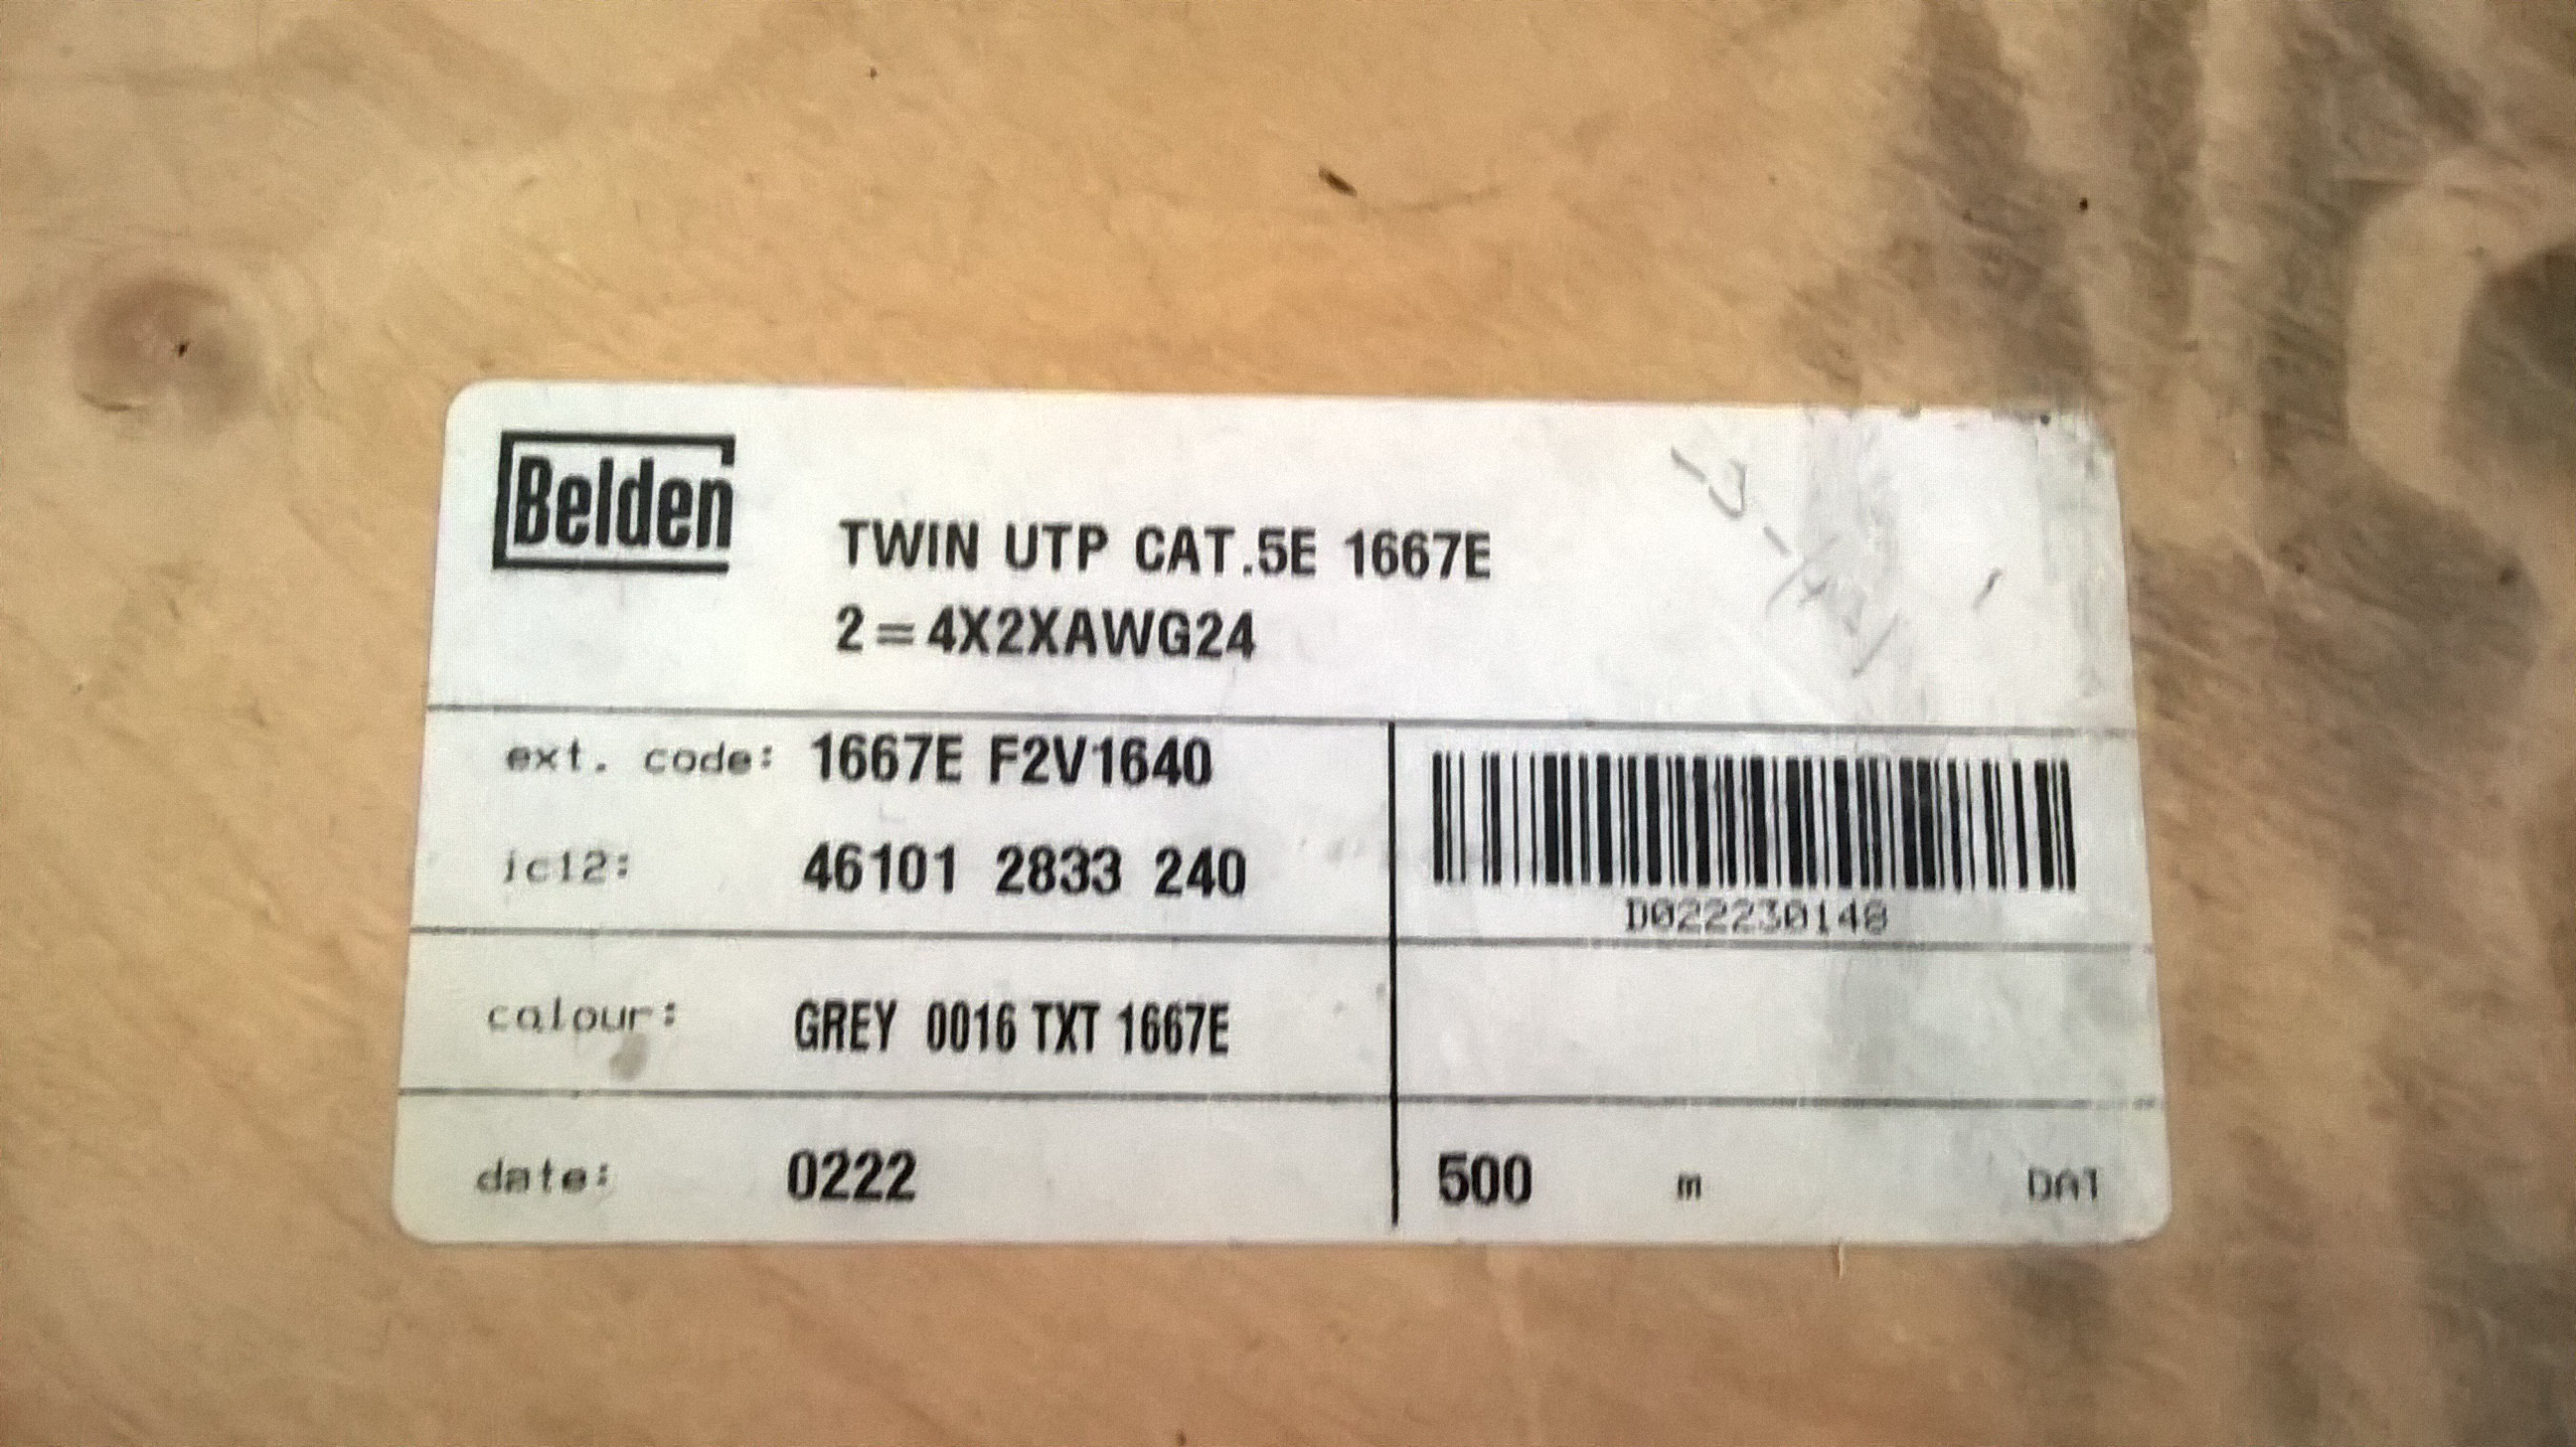
\includegraphics[scale=0.1]{Radar/16}}
\caption{Coaxial cable}
\end{figure}
\item Connection box
\item Resistor box
\item $100\Omega$ resistor and $30\mu F$ capacitor
\begin{figure}[H]
\centerline{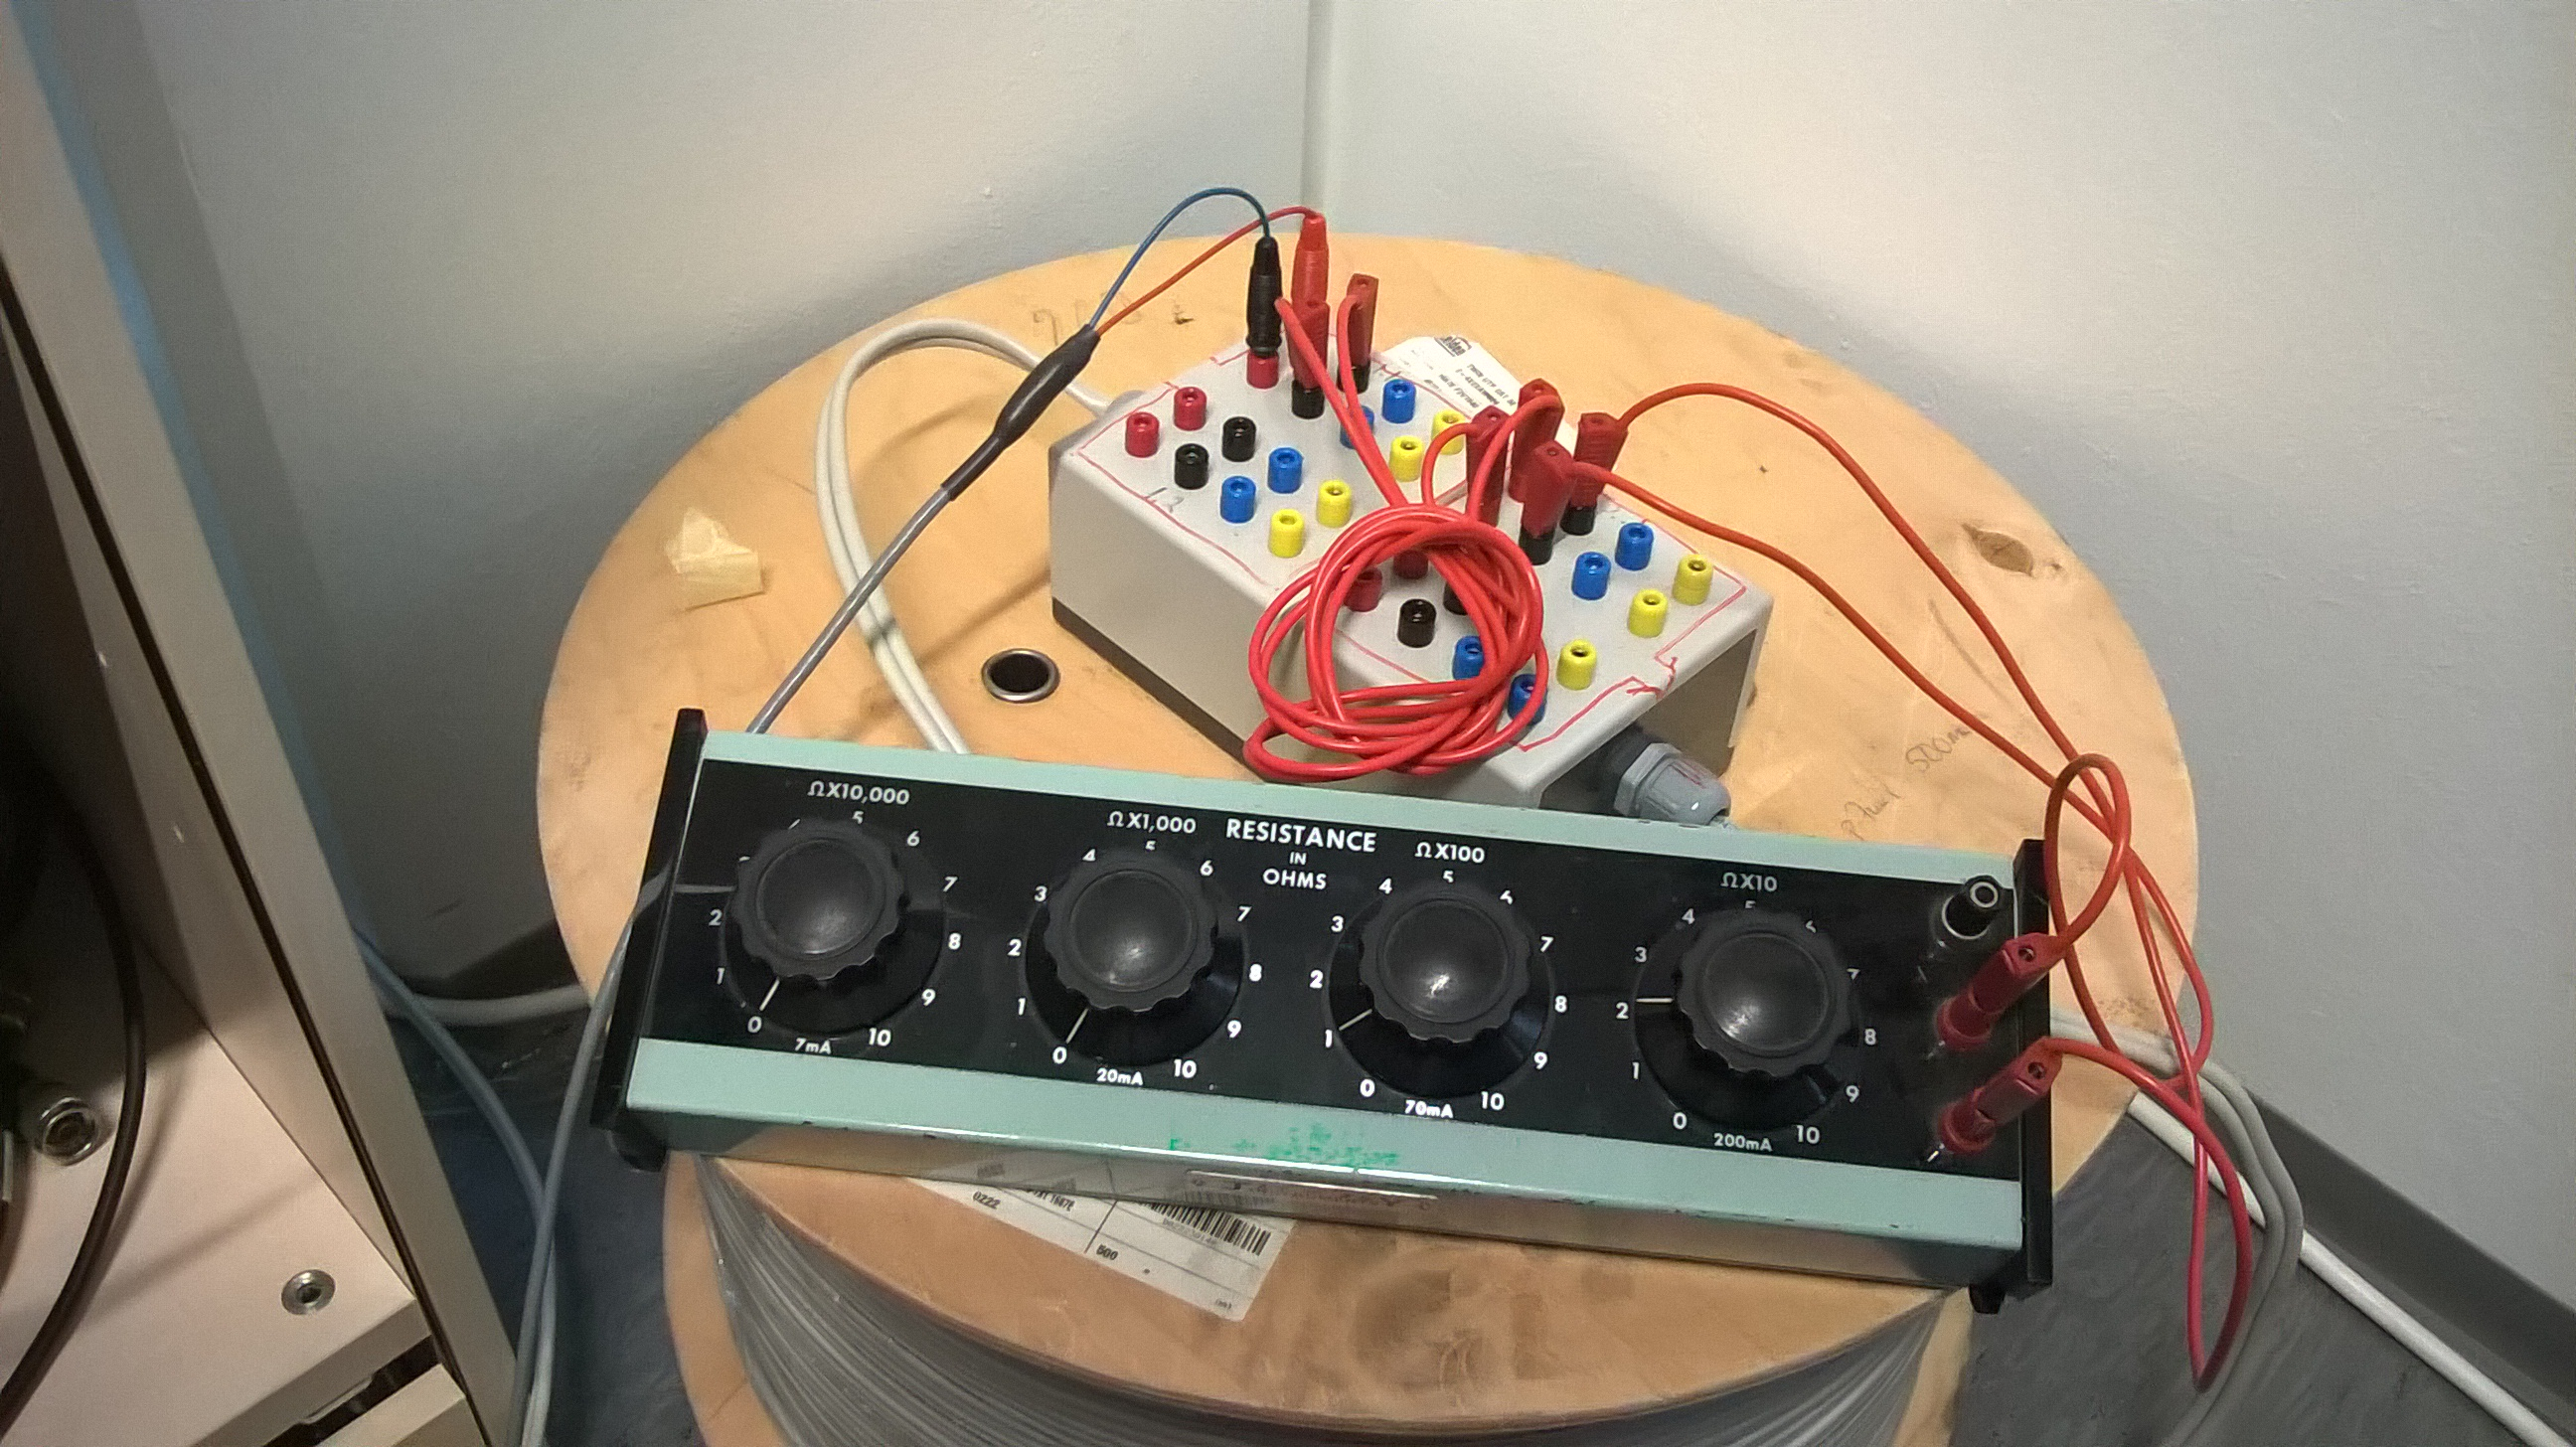
\includegraphics[scale=0.1]{Radar/15}}
\caption{Connection and resistors boxes}
\end{figure}
\item different kinds of wire
\end{itemize}
\section{Process of work}
The technique is used to determine the location of the fault, it is also possible to use the graph to estimate an impedance which made the circuit short.
\subsection{Distance}
\subsubsection{Measurements and calculation}
We have put the resistor on 500m distance from sensor and found the settings when the peak was on the center(as close as it was possible) of our scale, it gives as an opportunity to make the most accurate calculations of the length of our cable and location of the resistor. The scale was $20\mu s$ from one side to another.
$$
2d= \Upsilon T \rightarrow d=\dfrac{\Upsilon T}{2}\\
$$
$$
\begin{rcases}
\Upsilon=0.33c=0.33 \cdot 3m/s \cdot 10^8 \\
T=20 \mu s=2 \cdot10^{-5}s\\
d=\dfrac{\Upsilon T}{2}
\end{rcases}  \rightarrow d=\frac{0.33 \cdot 10^8 \cdot 3m/s \cdot 2s \cdot 10^{-5}}{2}=990m
$$
\begin{figure}[H]
\centerline{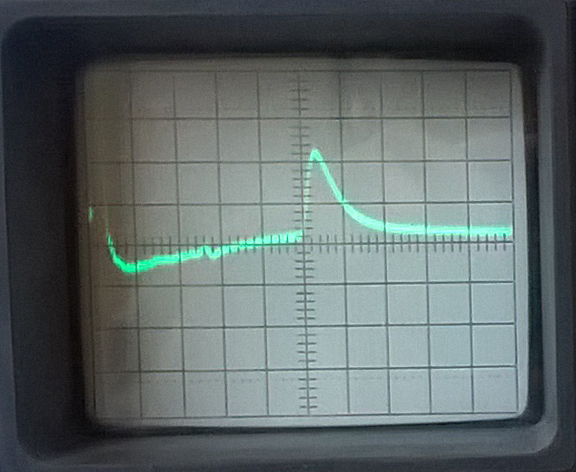
\includegraphics[scale=0.5]{Radar/6}}
\caption{1km of coaxial cable, $120 \Omega$ Resistor}
\end{figure}
The peak is produced by reflection of the $120 \Omega$ resistor, it is placed very close to the centrer of the scale, let us suppose that it is about 52\% from the left side. In an according with formula above d is directly proportional to T, T is changed by 52\%, it means that we can get the distance from the sensor to the resistor by multiplication of the whole distance by the percent.
$$
d=990m\cdot0.52=514m
$$
\subsubsection{Results}
 In an according with our calculation the distance between sensor and resistor is 514m and whole length is 990m, in real life they are 500m and 1km correspondingly
\subsection{Impedance for resistor}
\subsubsection{Measurements and calculation}
It is also possible to calculate impedance by eq. 1
$$
\rho=\frac{R_L-Z_0}{R_L+Z_0}(1)
$$
The scale don't have any marking, that's why it should be calibrated by know value of $\rho$, after the actual measurement.\\\\
On the figure 4 shows as the graph with peak equal -3 cells. The figure 3 shows as calibration measurements for the settings of the TDR. In an according with data-sheet(look materials) an impedance of the cable is $Z_0=1km \cdot 100\Omega/km$
$$
\rho=\frac{R_L-Z_0}{R_L+Z_0}=\frac{120\Omega-100\Omega}{120\Omega+100\Omega}=\frac{20}{220}
$$
$$
\rho=\frac{1}{11}
$$
The peak is around 2 cells. $\rightarrow \rho/cell=\frac{1}{22}$.
This price of the cell helps as to calculate the impedance of the resistor. There is -3 cell $\rightarrow \rho=-\frac{3}{22}$.
$$
-\frac{3}{22}=\frac{R_L-100\Omega}{R_L-100\Omega}
$$
$$
-\frac{3}{22} \cdot R_L-\frac{3}{22} \cdot 100=R_L-100
\rightarrow
-\frac{25}{22} \cdot R_L= -\frac{19}{22} \cdot 100
$$
$$
25R_L=1900 \rightarrow R_L\approx76\Omega
$$
\begin{figure}[H]
\centerline{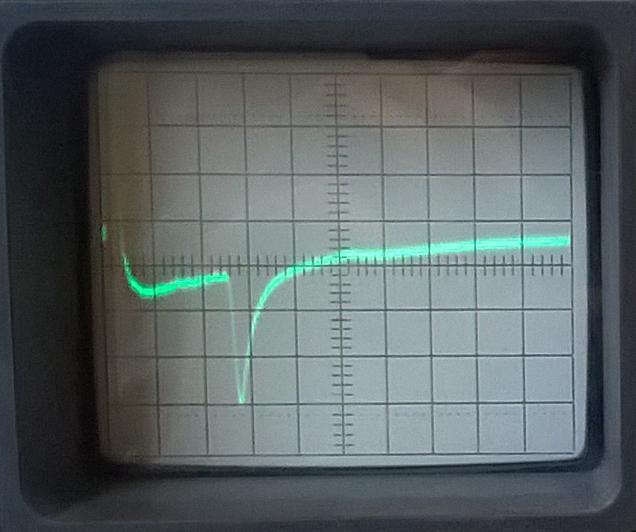
\includegraphics[scale=0.4]{Radar/7}}
\caption{Short-circuit 500m, resistor $100 \Omega$}
\end{figure}
\subsubsection{Results}
 In an according with our calculation the resistor has $76\Omega$ and in real life they are
  $100\Omega$
\subsection{Impedance for capacitor}
\begin{figure}[H]
\centerline{
\includegraphics[scale=0.25]{Radar/13}}
\caption{1km of coaxial cable, $120 \Omega$ Resistor, scale for $50\mu$ F capacitor's reflection}
\end{figure}
At the same way we can calculate an impedance if the circuit is shorted by capacitor. As previously our calibration $\rho=\frac{1}{11}$, but the peak is only half of cell high now, and our reflection peak is -1.5. \\\\
\begin{figure}[H]
\centerline{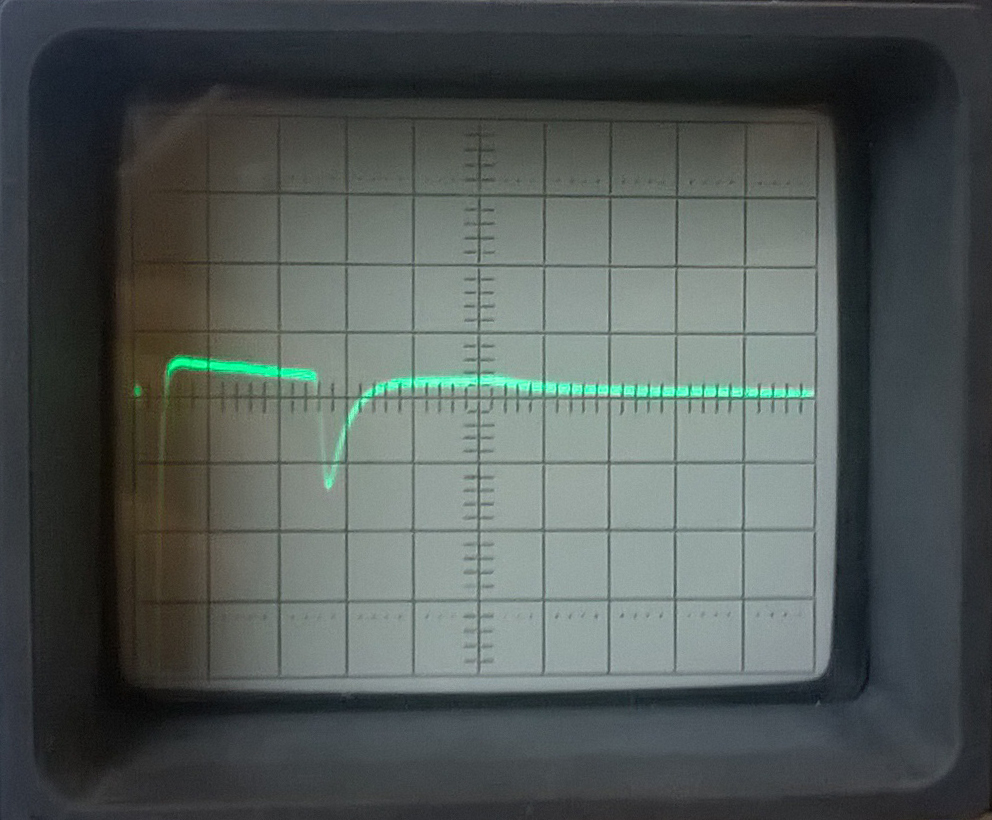
\includegraphics[scale=0.3]{Radar/11}}
\caption{Short-circuit 500m, capacitor $50 \mu F$}
\end{figure}
So the reflection coefficient of peak is $-\frac{3}{11}$.
$$
-\frac{3}{11}=\frac{R_L-100\Omega}{R_L-100\Omega}
$$
$$
-\frac{3}{11} \cdot R_L-\frac{3}{11} \cdot 100=R_L-100
\rightarrow
-\frac{14}{11} \cdot R_L= -\frac{8}{11} \cdot 100
$$
$$
14R_L=800 \rightarrow R_L\approx57\Omega
$$
It is possible to calculate the capacitance form an impedance by the formula $X=\frac{1}{C \omega}$, where X is an impedance and $\omega$ is angular velocity. We know that the frequency in power line is $50Hz$ and $\omega=2 \pi f$ from this facts we can get the formula below.
 $$C=\frac{1}{2\pi Xf}$$
 And now we have enough data to calculate capacitance.
 $$
 C=\frac{1}{2 \pi\cdot 57\Omega \cdot 50Hz•}\approx55 \mu F
 $$
 \subsubsection{Result}
 During our calculation we have found that the capacitance is $55\mu F$, the result is close enough, because the capacitor was $50\mu F$. It is the most accurate calculation for all the lab work.
\section{Conclusion}
I think that the result is well for so inaccurate measurements technique. I am not going to calculate errors because in any case they would be huge, actually it is not measurement technique it is estimation one, the method was only created to reduce searching area, because it is very difficult to find exact location in the cable which is underground.
\end{document}
